\documentclass[a4paper]{article}

\usepackage{amsmath}
\usepackage{hyperref}
\usepackage{biblatex}
\usepackage{enumerate}
\usepackage{graphicx}
\usepackage{stmaryrd}
\addbibresource{refs.bib}

\begin{document}

\author{Jack Daniels \\
  \href{mailto:jack.daniels@chalmers.se}{jack.daniels@chalmers.se}
  \and
  Emmett Brown \\
  \href{mailto:emmett.brown@gu.se}{emmett.brown@gu.se}
}
\title{DAT565/DIT407 Assignment 1}
\date{2024-01-11}

\maketitle

This is a template for a report for creating assignment reports for
the course \emph{Introduction to Data Science \& AI}.

\section*{Problem 1}

Please create sections that match the problems you are solving. If you
need figures or tables, do not remember to refer to them like so: we
see the results in Figure~\ref{fig:example1} and
Table~\ref{tbl:example2}.

If you need to cite external sources, do so by placing the literature
information in the file \texttt{refs.bib} in BibTeX format and use the
\texttt{\textbackslash{}cite} command, like so: In the first
assignment, we use data from SCB~\cite{SCB:2023}.

The most convenient way to edit and compile this file is by using
\href{https://www.overleaf.com}{Overleaf}. However, if you have a
local \LaTeX installation, you can compile the file by issuing the
following commands:\\
\texttt{\$ pdflatex report.tex} \\
\texttt{\$ biber report} \\
\texttt{\$ pdflatex report.tex} \\
\texttt{\$ pdflatex report.tex} \\

\begin{figure}[htb]
  \begin{center}
    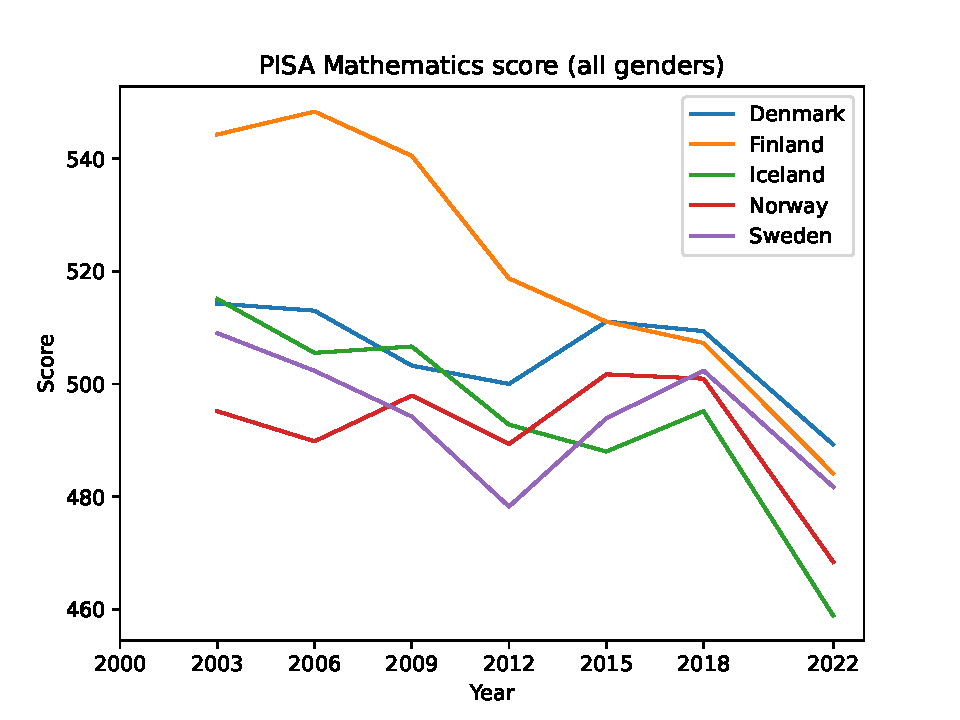
\includegraphics[width=\textwidth]{pisa_mathematics_in_nordic_countries.pdf}
    \caption{PISA mathematics score in different nordic countries.}
    \label{fig:example1}
  \end{center}
\end{figure}

\begin{table}[htb]
  \begin{center}
    \caption{Nordic countries' area and population.}
    \label{tbl:example2}
    \begin{tabular}{l|rr}
      Country & Area (km$^2$) & Population \\\hline
      Denmark & 43,094 & 5,935,619 \\
      Finland & 338,145 & 5,614,571 \\
      Iceland & 103,125 & 387,800 \\
      Norway  & 385,207 & 5,488,984 \\
      Sweden  & 450,295 & 10,540,886 \\
    \end{tabular}
  \end{center}
\end{table}


\printbibliography

\end{document}
